\section{Model 1:Fungi Population Prediction Model}
\subsection{Competitive Lotka-Volterra equations}
	Our final goal of modeling is to simulate the degradation of plant material by fungi. Therefore, at first we should resolve how will fungi community evolve under given environment conditions. In our model, there is competition between different fungi species rather than predator-prey relationship.  And all these species compete for common resource, which are plant material. Thus, the Competitive Lotka-Volterra Equations (CLV) is adopted to depict fungi population dynamics. 

	The N-species CLV equations are: 
	\begin{align}
		\frac{\textrm d S_i}{\textrm d t}=r_iS_i(1-\frac{\sum_{j=1}^N\alpha_{ij}S_j}{K_i})
	\end{align}  

	where $S_i(t)$ is the size of the $i$-th population at a given time, $N$ is the total number interacting species, $r_i$ is inherent per-capita growth rate of $i$-th species, $\alpha_{ij}$ represents the effect species j has on the population of species i and $K_i$ is the carrying capacity of $i$-th species.


 
\subsection{Parameter Estimation and Definition of CLV Equations}
\subsubsection{Carrying Capacity: $K$}
	In a given patch of land,  the overall living space is fixed. Therefore, the carrying capacity of one species is proportional to its density:
	\begin{align}
		K_i \propto \rho_i
	\end{align}

	In our model there is no need to know the specific value of $K_i$, only the relative value matters.
	
\subsubsection{Inherent Per-capita Growth Rate: $r_i$}
	According to definition, we have:
	\begin{align}
		r_i \propto v_{\text{extension}}
	\end{align}
            
\subsubsection{Interaction Parameter: $\alpha_{ij}$}

	$\alpha_{ij}$ means the effect species j has on the population of species i. Here we use the competitive rank of fungi, which is accessible to us, to define the parameter. And two rules must be followed:
	\begin{itemize}
		\item All $\alpha$ values are positive
		\item $\alpha_{ij}=1$ when $i=j$
	\end{itemize}

	Therefore, we assume:
	\begin{align}
		\alpha_{ij}=\exp(1-\frac{n_i}{n_j})	
	\end{align}

	Where $n_i$ represents the competitive rank.(The bigger the $n_i$, the higher the ranking)


\subsection{Results}
3 kinds of fungi were selected.(Identifier:1,4,6. Refer to the appendix for detail traits) 

%-----------------------------------------------------------------
\iffalse
	6 kinds of fungi were selected. Refer to the appendix for details. 
	The computation was under such conditions:
 
	\begin{align}
    	T=22^{\circ}\text C,\ M=-0.5\text{MPa}\nonumber   
	\end{align}

	and the population evolution with time is shown in Figure \ref{fig:result1}

	\begin{figure}[H]
    	\centering
	    \includegraphics[width=.6\textwidth]{25_05.png}
    	\caption{The result of Model 1}\label{fig:result1}
    \end{figure}
 \fi
%-----------------------------------------------------------------  
\begin{figure}[htbp]
\centering
\subfigure[$T = 22^{\circ}\text C,\ M = -0.25\text{MPa}$]{
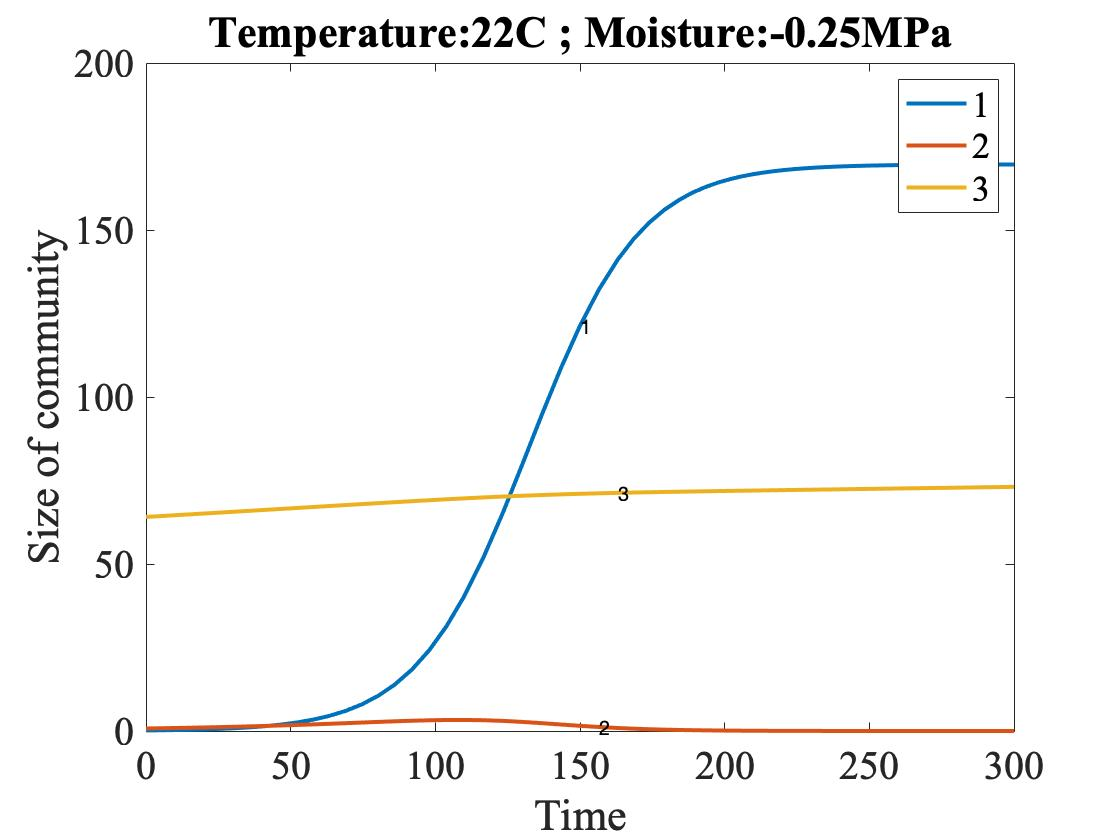
\includegraphics[width=6cm]{growth3_22_025.jpg}
%\caption{fig1}
}
\quad
\subfigure[$T = 25^{\circ}\text C,\ M = -0.5\text{MPa}$]{
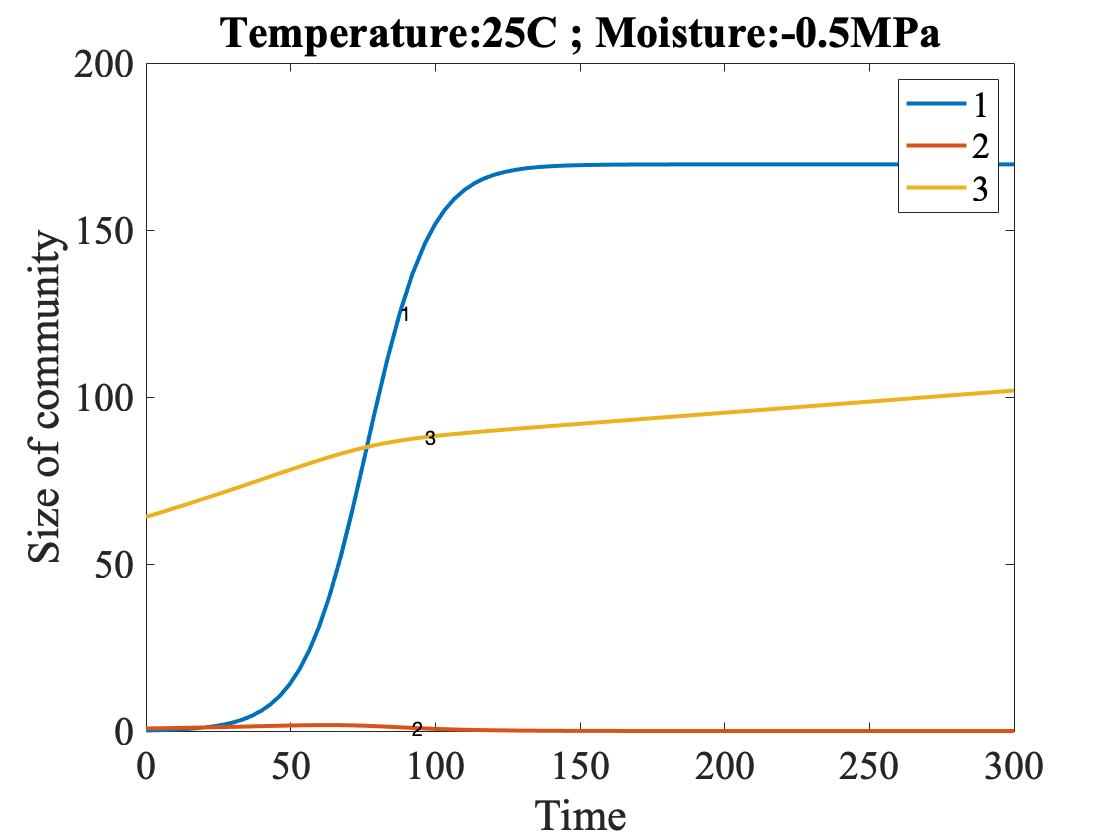
\includegraphics[width=6cm]{growth3_25_05.jpg}
}
\quad
\subfigure[$T = 25^{\circ}\text C,\ M = -2.5\text{MPa}$]{
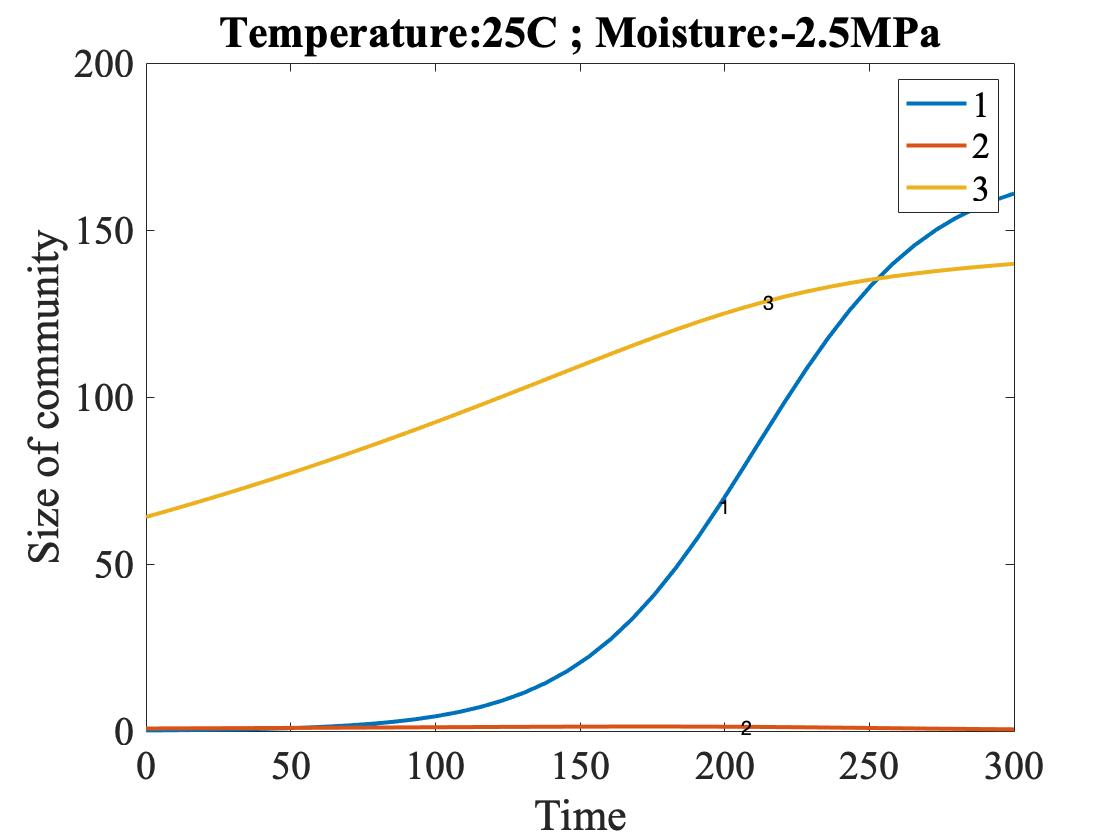
\includegraphics[width=6cm]{growth3_25_25.jpg}
}
\quad
\subfigure[$T = 33^{\circ}\text C,\ M = -0.5\text{MPa}$]{
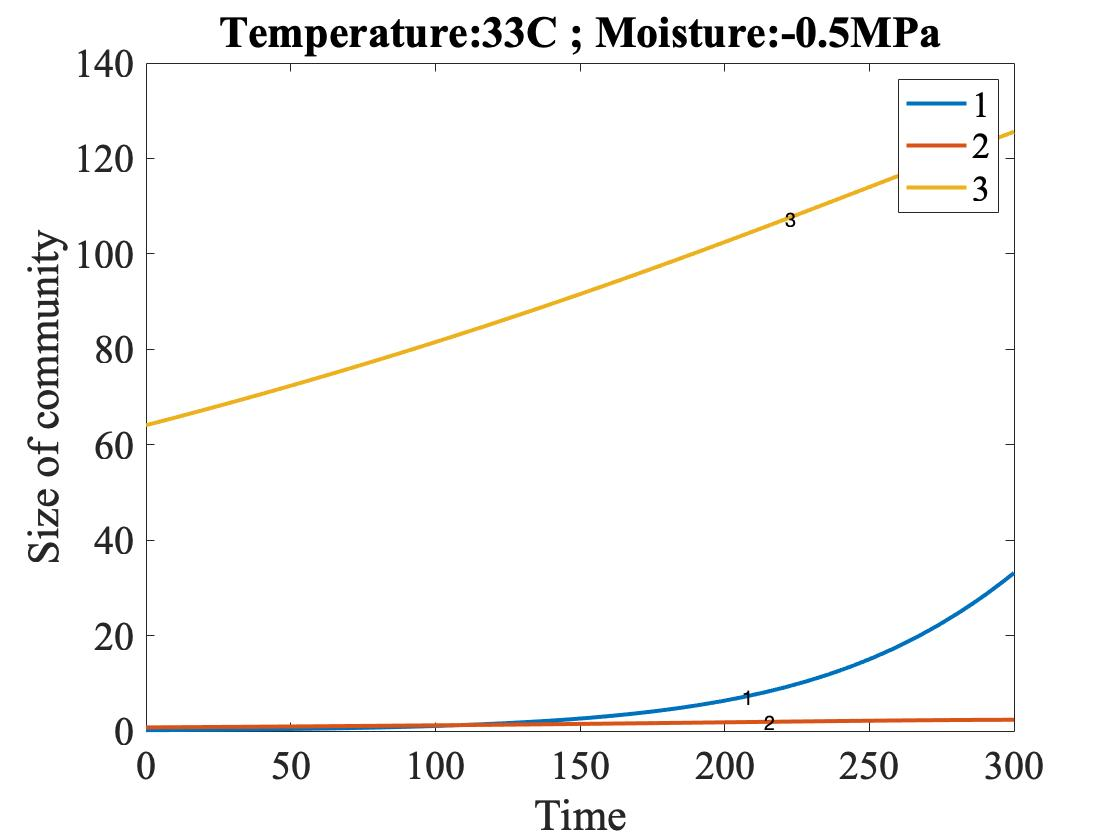
\includegraphics[width=6cm]{growth3_33_05.jpg}
}
\caption{Population Development}
\end{figure}



  
\subsection{Discussion}




















